\documentclass[conference]{IEEEtran}
\IEEEoverridecommandlockouts
\usepackage{cite}
\usepackage{amsmath,amssymb,amsfonts}
\usepackage{algorithmic}
\usepackage{graphicx}
\usepackage{textcomp}
\usepackage{xcolor}
\usepackage{booktabs}
\usepackage{multirow}
\usepackage[normalem]{ulem}
\useunder{\uline}{\ul}{}
\usepackage[percent]{overpic}



\usepackage[acronym]{glossaries}
\newacronym{MOO}{MOO}{Multi-Objective Optimization}
\newacronym{MOPs}{MOPs}{Multi-Objective Optimization Problems}
\newacronym{MOEAs}{MOEAs}{Multi-Objective Evolutionary Algorithms}
\newacronym{HV}{HV}{Hypervolume}

\newacronym{QR}{QR}{Quantile Regression}
\newacronym{NSGA-II}{NSGA-II}{Non-dominated Sorting Genetic Algorithm II}
\newacronym{RBFNs}{RBFNs}{Radial Basis Function Networks}
\newacronym{XGBoost}{XGBoost}{eXtreme Gradient Boosting}
\newacronym{GBDT}{GBDT}{Gradient Boosting Decision Trees}
\newacronym{NN}{NN}{Neural Network}
\newacronym{MSE}{MSE}{Mean Squared Error}
\newacronym{PMV}{PMV}{Predicted Mean Vote}
\newacronym{ML}{ML}{Machine Learning}
\newacronym{MCD}{MCD}{Monte Carlo Dropout}
\newacronym{BNN}{BNN}{Bayesian Neural Network}
\newacronym{DR}{DR}{Dual-Ranking}
\newacronym{GPR}{GPR}{Gaussian Process Regression}
\newacronym{PF}{PF}{Pareto Front}

\def\BibTeX{{\rm B\kern-.05em{\sc i\kern-.025em b}\kern-.08em
    T\kern-.1667em\lower.7ex\hbox{E}\kern-.125emX}}
\begin{document}

\title{A Study of Offline Data-Driven Multi-Objective Optimization for Real-World Problems}

\iffalse
\author{\IEEEauthorblockN{1\textsuperscript{st} Huanbo Lyu}
\IEEEauthorblockA{\textit{Computer Science} \\
\textit{University of Birmingham}\\
Birmingham, UK \\
hxl099@student.bham.ac.uk}
~\\
\and
\IEEEauthorblockN{2\textsuperscript{nd} James Andrews}
\IEEEauthorblockA{\textit{School of Mathematics} \\
\textit{University of Birmingham}\\
Birmingham, UK \\
j.w.andrews@bham.ac.uk}
~\\
\and
\IEEEauthorblockN{3\textsuperscript{rd} Daniel Herring}
\IEEEauthorblockA{\textit{School of Mathematics} \\
\textit{University of Birmingham}\\
Birmingham, UK \\
d.g.herring@bham.ac.uk}
~\\
\and
\IEEEauthorblockN{4\textsuperscript{th} Fabian Spill}
\IEEEauthorblockA{\textit{School of Mathematics} \\
\textit{University of Birmingham}\\
Birmingham, UK \\
f.spill@bham.ac.uk}
~\\
\and
\IEEEauthorblockN{5\textsuperscript{th} Shuo Wang*}
\IEEEauthorblockA{\textit{Computer Science} \\
\textit{University of Birmingham}\\
Birmingham, UK \\
s.wang.2@bham.ac.uk}
}
\fi

\author{\IEEEauthorblockN{Anonymous submission}}


\maketitle

\begin{abstract}
Many real-world Multi-objective Optimization Problems (MOPs) do not have explicit mathematical formulations of their objective functions. Data-driven multi-objective evolutionary algorithms (MOEAs) address this limitation by using surrogate models to approximate objective values and evolutionary algorithms as optimizers. As it is often difficult to obtain real objective values, the effectiveness of this type of approach is still unclear. This paper conducts an in-depth study of the existing offline data-driven MOEAs, including seven classic and eight uncertainty-aware approaches, on eight real-world benchmark problems. The results show that TabPFN+NSGA-II, GPR-Mat\'ern+NSGA-II, and GPR-Mat\'ern+NSGA-II+DR achieve the top-three overall performance by balancing predictive accuracy (MSE), surrogate-real evaluation consistency, and optimization performance (HV). These three methods are then applied to a flexible building space optimization problem. Although the real objective values of the obtained solutions are unknown, these methods still reveal some similar patterns in room configurations.



\end{abstract}

\begin{IEEEkeywords}
Data-driven multi-objective optimization, Data-driven evolutionary algorithm, Building space optimization
\end{IEEEkeywords}

\section{Introduction}
Many real-world problems can be formulated as \gls{MOPs} involving multiple conflicting objectives. In practice, however, some objective functions lack explicit analytical formulations or simulation models for direct evaluation~\cite{ddeo_rvea}. In such cases, surrogate models are often used to approximate the objectives, and data-driven \gls{MOEAs} combine the predictive capability of surrogate models with the search ability of evolutionary algorithms to identify high-quality solutions. These methods have been successfully applied to various real-world optimization tasks, including airfoil design~\cite{ddeo_2}, trauma systems~\cite{ddeo_1}, energy systems, and smart building optimization~\cite{building_opt, building_opt2}.

Unlike online data-driven \gls{MOEAs} or surrogate-assisted \gls{MOO}, where real evaluations are available during optimization and additional sampled data points can be evaluated to improve the surrogate models, offline data-driven \gls{MOEAs} cannot query candidate solutions on the fly~\cite{ddeo_ibea,ddeo_rvea}. They rely on pre-collected datasets to train surrogate models for prediction. For example, in smart building optimization, building energy consumption is difficult to calculate directly. Historical energy-consumption data can be collected together with indoor and outdoor environmental data to train surrogate models.

In offline data-driven \gls{MOO} settings, surrogate approximations introduce uncertainty, which can significantly affect optimization performance by misleading the search process~\cite{ddeo_2}. To address this issue, several uncertainty-aware methods have been proposed~\cite{ddeo_ibea, ddeo_rvea, ddeo-TGPR, lyu_dual_ranking}. These methods rely on uncertainty estimates from surrogate modeling methods, such as \gls{GPR}~\cite{gaussian_kernel}, \gls{QR}~\cite{quantile_regression}, and \gls{BNN}~\cite{bnn}. The uncertainty estimates are then used directly in the optimization process to reduce the risk of misleading the search.

Although many approaches have been proposed, it is unclear how they perform in real-world settings, because the ground truth is often unavailable. This work first conducts comparative experiments on eight real-world benchmark problems to evaluate uncertainty-aware and standard data-driven \gls{MOEAs} using different surrogate models. These benchmark problems have true objective values for effectiveness and reliability comparison. The methods that achieve superior benchmark performance are then applied to a real-world building space optimization problem, where the true objective values are unknown. Although real evaluations cannot be conducted, we observe some similar patterns in the obtained room configurations.

The results of this study provide an empirical basis for method selection in offline data-driven multi-objective optimization. When real evaluations are available on real-world benchmark problems, different metrics can be adopted to compare the performance of the methods, and TabPFN combined with NSGA-II achieves the best overall performance. In contrast, when only surrogate-based evaluation is available, as in the real-world building space optimization problem, the obtained fronts may show different patterns across methods. The corresponding room configurations can still exhibit similar patterns.



\section{Method}
\subsection{Multi-Objective Optimization}
The \gls{MOPs} can be formulated as follows:
\begin{align}\label{eq:mops}
\text{minimize }& \boldsymbol{f}(\mathbf{x}) = \left(f_1(\mathbf{x}), f_2(\mathbf{x}), \ldots, f_T(\mathbf{x})\right) \nonumber \\
\text{subject to }& \mathbf{x} \in S ,
\end{align}
where $\mathbf{x}$ is the decision vector, $T \geq 2$ denotes the number of objectives, and $S$ is the feasible region in the decision space. A solution $\mathbf{x}_1 \in S$ dominates another solution $\mathbf{x}_2 \in S$, indicated as $\mathbf{x}_1 \prec \mathbf{x}_2$, if $f_t(\mathbf{x}_1) \leq f_t(\mathbf{x}_2)$ for all $t=1,\ldots,T$ and $f_t(\mathbf{x}_{1}) < f_t(\mathbf{x}_{2})$ for at least one $t = 1,\ldots,T$. The set of non-dominated feasible solutions is the Pareto set, and their objective values constitute the Pareto front.

\subsection{Offline Data-Driven Multi-Objective Optimization}
In real-world \gls{MOPs}, the objective functions may not have explicit mathematical expressions. The objective values can be approximated by surrogate models $\mathcal{M}$ trained on a pre-collected dataset $\mathcal{D} = \{(x_i, y_i)\}_{i=1}^{N}$. These surrogate models are then used to evaluate candidate solutions $\mathbf{x}$ during optimization, while real evaluations remain unavailable.

The offline data-driven \gls{MOEAs} tested in this work are summarized in Table~\ref{tab:methods_table}. For uncertainty-aware methods, we select GPR, QR, and BNN, which quantify uncertainty from different perspectives. For standard surrogates, we choose popular regression methods, including XGBoost, ensemble-based regression method Autogluon-Tabular, and pre-trained method TabPFN.

\begin{table*}[htbp]
\centering
\caption{Summary of the surrogate models and optimizers compared in the experiments.}
\label{tab:methods_table}
\small
\begin{tabular}{@{}ll@{}}
\toprule
\textbf{Surrogate models} & \textbf{Optimizers} \\
\midrule
GPR-RBF~\cite{gaussian_kernel} & NSGA-II~\cite{nsga_ii}, NSGA-II+DR~\cite{lyu_dual_ranking} \\
GPR-Mat\'ern~\cite{kernel_Matern_52} & NSGA-II, NSGA-II+DR \\
QR~\cite{ml_autogluon} & NSGA-II, NSGA-II+DR \\
BNN~\cite{pyro} & NSGA-II, NSGA-II+DR \\
\midrule
XGBoost~\cite{opt_xbgoost} & NSGA-II \\
WeightedEnsemble\_L2~\cite{ml_autogluon} & NSGA-II \\
TabPFN~\cite{tabpfn} & NSGA-II \\
\midrule
\multicolumn{2}{@{}l@{}}{\textbf{Surrogate models + Optimizers}} \\
\midrule
\multicolumn{2}{@{}l@{}}{
Prob-RVEA~\cite{ddeo_rvea}, 
Prob-MOEA/D~\cite{ddeo_rvea}, 
TGPR-MO~\cite{ddeo-TGPR}, 
DDMOEA/GAN~\cite{ddea_gan}
} \\
\bottomrule
\end{tabular}
\end{table*}




\subsubsection{Surrogate Models}
The GPR assumes that observations are jointly Gaussian distributed. The prediction $\hat{y}$ at the point $\mathbf{x}$ can be expressed as:
\begin{equation}
\hat{y} = \mu(\mathbf{x}) + \epsilon(\mathbf{x}),
\end{equation}
where $\mu(\mathbf{x})$ represents the mean function, and $\epsilon(\mathbf{x})$ is a stochastic term with covariance determined by $k(\mathbf{x}, \mathbf{x}')$. The Gaussian kernel \cite{gaussian_kernel}, defined as:
\begin{equation}
k(\mathbf{x}, \mathbf{x}') = \sigma_f^2 \exp \left( -\frac{1}{2} r^2(\mathbf{x}, \mathbf{x}') \right), 
\end{equation}
where \(r^2(\mathbf{x}, \mathbf{x}')\) denotes the squared distance between two input samples. The Automatic Relevance Determination (ARD) Mat\'ern \(5/2\) kernel \cite{kernel_Matern_52} is given by: 
\begin{equation}
\begin{aligned}
k_{\mathrm{M52}}(\mathbf{x}, \mathbf{x}')
&=
\sigma_f^2
\left(
1 + \sqrt{5 r^2(\mathbf{x}, \mathbf{x}')}
+ \frac{5}{3} r^2(\mathbf{x}, \mathbf{x}')
\right) \\
&\quad \cdot
\exp
\left(
-\sqrt{5 r^2(\mathbf{x}, \mathbf{x}')}
\right).
\end{aligned}
\end{equation}
Compared with the Gaussian kernel, the Mat\'ern \(5/2\) does not make the covariance function unrealistically smooth \cite{ddeo-TGPR}.

The \gls{QR} estimates the conditional quantile (\emph{e.g.} median) of the target variable. For a given quantile level $\tau \in (0, 1)$, the coefficient is defined as:
\begin{align}
\hat{\boldsymbol{\beta}}_\tau = \arg\min_{\boldsymbol{\beta}} \sum_{i=1}^n \rho_\tau \left( y_i - \mathbf{x}_i^\top \boldsymbol{\beta} \right),
\end{align}
where $\rho_\tau(u)$ denotes the ``check function'' \cite{pinball_loss} defined as:
\begin{align}
\rho_\tau(u) =
\begin{cases}
\tau u, & \text{if } u \geq 0 \\
(1 - \tau) u, & \text{if } u < 0.
\end{cases}
\end{align}

The \gls{BNN} treats the network weights as probability distributions and approximates the posterior distribution $p(\mathbf{w} \mid \mathcal{D})$ over weights $\mathbf{w}$ using variational inference. Given an input $\mathbf{x}$, the predictive distribution can be estimated through Monte Carlo sampling as:
\begin{align}
p(y \mid \mathbf{x}) \approx \frac{1}{S} \sum_{s=1}^{S} p(y \mid \mathbf{x}, \mathbf{w}^{(s)}), \quad \mathbf{w}^{(s)} \sim q(\mathbf{w}),
\end{align}
where $q(\mathbf{w})$ denotes the variational posterior.

The XGBoost is an efficient gradient boosting framework based on regression trees. It approximates the target function by additively combining $K$ regression trees:
\begin{equation}
\hat{y}_i = \phi(\mathbf{x}) = \sum_{k=1}^{K} f_k(\mathbf{x}),
\quad f_k \in \mathcal{F},
\end{equation}
where \(\mathcal{F}\) denotes the space of regression trees. 
The model is trained by minimizing a regularized objective function:
\begin{equation}
\mathcal{L}(\phi)
=
\sum_{i=1}^{N} l(y_i,\hat{y}_i)
+
\sum_{k=1}^{K}
\left(
\gamma T_k
+
\frac{1}{2}\lambda
\sum_{j=1}^{T_k} w_{kj}^{2}
\right),
\end{equation}
where \(l(\cdot)\) is the training loss, \(T_k\) is the number of leaves in the \(k\)-th tree, \(w_{kj}\) is the score of the \(j\)-th leaf, and \(\gamma\) and \(\lambda\) are regularization parameters. 
By combining multiple weak regression trees and explicitly penalizing model complexity, XGBoost can capture nonlinear input-output relationships while reducing overfitting.


The WeightedEnsemble\_L2 is an ensemble model in AutoGluon-Tabular that learns optimal weights for combining base learners through L2-regularized weighted averaging. Its prediction $\hat{y}$ is given by
\begin{equation}
\hat{y} = \sum_{m=1}^M \alpha_m \hat{y}_{m}
\end{equation}
where $\alpha_m$ is the learned weight and $\hat{y}_{m}$ is the prediction of the $m$-th base learner.

TabPFN is a transformer-based tabular prediction model that performs in-context learning for small tabular datasets. Instead of training a task-specific model, TabPFN is pre-trained on a large collection of synthetic tabular datasets generated from prior distributions over possible learning problems. The model directly conditions on the observed input-output pairs and produces predictions for unseen samples. This enables fast inference without task-specific training. 

\subsubsection{Optimizers}
\gls{NSGA-II}~\cite{nsga_ii} is employed as the main optimization algorithm. It optimizes multiple objectives and maintains solution diversity through non-dominated sorting, crowding distance, and elitism. In this work, uncertainty estimates obtained from the surrogate models described above are incorporated into the optimization process using the \gls{DR} strategy~\cite{lyu_dual_ranking}. This strategy considers the non-dominated front based on both the surrogate-based objective function $f_{\text{sur}}$ and the uncertainty-aware objective function $f_{\text{UA-sur}}$.


\subsubsection{Offline Data-Driven Multi-Objective Evolutionary Algorithms}
The surrogate models and optimizers introduced above are combined to form the following methods: GPR-RBF+NSGA-II, GPR-RBF+NSGA-II+DR, GPR-Mat\'ern+NSGA-II, GPR-Mat\'ern+NSGA-II+DR, QR+NSGA-II, QR+NSGA-II+DR, BNN+NSGA-II, BNN+NSGA-II+DR, XGBoost+NSGA-II, WeightedEnsemble\_L2+NSGA-II, and TabPFN+NSGA-II.

Other baseline offline data-driven \gls{MOEAs} include Prob-RVEA, Prob-MOEA/D, TGPR-MO, and DDMOEA/GAN, which combine surrogate modeling with optimization. Prob-RVEA uses GPR-based uncertainty estimation and uncertainty-aware selection to guide reference-vector-based search in offline data-driven settings. Prob-MOEA/D is a probabilistic decomposition-based evolutionary algorithm that incorporates surrogate uncertainty estimated by GPR. TGPR-MO combines GPR with regression trees to partition the decision space and build local GPR models, thereby reducing the computational burden of full GPRs for larger datasets. DDMOEA/GAN~\cite{ddea_gan} uses the discriminator and generator mechanisms of a generative adversarial network (GAN) for trust-aware evaluation and data augmentation, respectively.

\section{Experiments}
\subsection{Experimental Setup}
\subsubsection{Benchmark Problems}
The evaluation includes 8 real-world bi-optimization problems, including Truss2D~\cite{truss2d}, Welded Beam~\cite{welded_beam}, RE21-25 \cite{xue2024offline} and MO-Portfolio. Truss2D is a structural truss design problem involving trade-offs between structural performance and material usage. Welded Beam is a classical constrained engineering design problem that optimizes beam geometry under stress and deflection constraints. RE21-25 are real-world constrained engineering benchmark problems covering representative mechanical and structural design tasks. MO-Portfolio is a financial portfolio optimization problem that balances return and risk in asset allocation.

\subsubsection{Offline Dataset}
Offline data are generated by Latin Hypercube Sampling (LHS)~\cite{sampling}. For each problem, 300 training samples are generated using a fixed training seed of 42. In addition, 100 validation samples and 100 test samples are generated for each benchmark problem. Unless otherwise specified, optimization experiments are repeated over 30 independent runs using random seeds from 1 to 30. 


\subsubsection{Surrogate Models and Optimizers}
Seven surrogate models are evaluated to identify suitable methods for the real-world case study. GPR-RBF and GPR-Mat\'ern are implemented in GPy using ARD RBF and ARD Matérn-$5/2$ kernels, respectively. \gls{QR} is implemented with AutoGluon-Tabular using random seed 42; the median prediction is used as the surrogate mean, and the 0.9 quantile is used for dual-ranking. \gls{BNN} is implemented in Pyro with two hidden layers of sizes 6 and 3, $\tanh$ activations, Normal weight priors with scale 0.5, target standardization, AutoDiagonalNormal, Trace-ELBO, and Adam~\cite{adam}. The learning rate is $5\times10^{-4}$, the maximum number of SVI steps is 50,000, validation is checked every 200 steps, early-stopping patience is 15 checks, the initial observation noise is 0.05, and 100 posterior predictive samples are used. XGBoost is implemented using the XGBoost regression backend, whereas WeightedEnsemble\_L2 is implemented with the default settings of AutoGluon-Tabular. TabPFN is accessed via the service API, and the regression task is implemented using the default TabPFNRegressor. Due to API call limitations, only five repeated runs are conducted for TabPFN.

The optimization framework is implemented in pymoo~\cite{pymoo}. For uncertainty-aware surrogates, both NSGA-II and NSGA-II+DR are tested, whereas the other surrogates are optimized only with standard NSGA-II. The population size is 100 and the number of generations is 100, resulting in 10,000 surrogate-based fitness evaluations. SBX crossover~\cite{opt-sbx} is used with probability 1.0 and distribution index $\eta=20$, and polynomial mutation is applied with probability $1/D$ and the same distribution index. We also include four previously proposed uncertainty-aware methods including Prob-RVEA~\cite{ddeo_rvea}, Prob-MOEA/D, TGPR-MO~\cite{ddeo-TGPR}, and DDMOEA-GAN~\cite{ddea_gan}.

\subsubsection{Performance Metrics} \label{sec: metrics}
The optimization results are evaluated by metrics including Mean Squared Error (MSE) and Hypervolume (HV). MSE$_{\mathrm{pre}}$ measures the predictive accuracy of each surrogate model, where lower values indicate better prediction performance. For the candidate solutions, MSE$_{\mathrm{sur\mbox{-}real}}$ measures the discrepancy between surrogate-predicted objective values and their corresponding real-evaluation objective values. Lower values indicate better consistency of surrogate-real evaluation. The optimization results is evaluated using the real-evaluation hypervolume, denoted as HV$_{\mathrm{real}}$~\cite{hypervolume}. Higher values indicate better optimization performance. Before calculating HV values, all objective values are normalized using min-max normalization~\cite{min_max}. The normalization bounds are selected based on the benchmark paper~\cite{xue2024offline} and the observed objective values obtained from both surrogate-based and real evaluations. The corresponding minimum and maximum values are reported in the Appendix. After normalization, a unified reference point of $(1.1, 1.1)$ is used. Since different surrogate models may produce different predicted objective ranges, surrogate-based hypervolume value is not used for fair comparison. 

The Friedman test~\cite{friedman} is applied to rank all candidate methods across the benchmark problems, and the three methods with the best average ranks are selected for further comparison. To further compare the top-three methods, Wilcoxon signed-rank tests~\cite{wilcoxon} are also conducted.


\subsection{Experimental Results}
Table~\ref{tab:benchmark_results} summarizes the optimization performance of different surrogate models and optimizers on eight real-world benchmark problems. The reported values are the mean and standard deviation over repeated runs. A mean value of zero may indicate that the algorithm failed to find any feasible solution. Table~\ref{tab:top3} reports the top-three methods selected by the Friedman test under two criteria including HV$_{\mathrm{real}}$ only, and a combined criterion based on MSE$_{\mathrm{pre}}$, MSE$_{\mathrm{sur\mbox{-}real}}$, and HV$_{\mathrm{real}}$. The HV$_{\mathrm{real}}$-only criterion focuses on optimization performance, as it directly evaluates the quality of the final solutions using real objective evaluations. In contrast, the combined criterion provides a more comprehensive assessment of surrogate models and optimizers by jointly considering prediction accuracy, surrogate-real evaluation consistency, and optimization quality.

Under HV$_{\mathrm{real}}$-only criterion shown in Table \ref{tab:top3}, TabPFN+NSGA-II obtains the best average rank, followed by QR+NSGA-II+DR and WeightedEnsemble\_L2+NSGA-II, suggesting that these methods are effective in generating high-quality Pareto solutions. Under the combined criterion, TabPFN+NSGA-II remains the best-performing method, while GPR-Mat\'ern+NSGA-II and GPR-Mat\'ern+NSGA-II+DR move into the second and third positions. This change indicates that although QR-based and ensemble-based methods can achieve competitive HV$_{\mathrm{real}}$, GPR-Mat\'ern-based methods provide a better balance between surrogate accuracy, surrogate-real consistency, and optimization performance. Since the combined criterion evaluates both the prediction model and the optimizer, TabPFN+NSGA-II, GPR-Mat\'ern+NSGA-II, and GPR-Mat\'ern+NSGA-II+DR are selected as the final top-three methods.




\begin{table*}[htbp]
\centering
\scriptsize
\setlength{\tabcolsep}{2pt}
\caption{Surrogate-model and optimizer results on eight real-world benchmark problems. For each metric column, the best and second-best results are highlighted in bold and underlined, respectively. Tied results are highlighted identically.}
\label{tab:benchmark_results}
\resizebox{\textwidth}{!}{%
\begin{tabular}{lcccccccccccc}
\toprule
Method & \multicolumn{3}{c}{RE21} & \multicolumn{3}{c}{RE22} & \multicolumn{3}{c}{RE23} & \multicolumn{3}{c}{RE24} \\
\cmidrule(lr){2-4} \cmidrule(lr){5-7} \cmidrule(lr){8-10} \cmidrule(lr){11-13}
 & MSE$_{\mathrm{pre}}$ & MSE$_{\mathrm{sur\mbox{-}real}}$ & HV$_{\mathrm{real}}$ & MSE$_{\mathrm{pre}}$ & MSE$_{\mathrm{sur\mbox{-}real}}$ & HV$_{\mathrm{real}}$ & MSE$_{\mathrm{pre}}$ & MSE$_{\mathrm{sur\mbox{-}real}}$ & HV$_{\mathrm{real}}$ & MSE$_{\mathrm{pre}}$ & MSE$_{\mathrm{sur\mbox{-}real}}$ & HV$_{\mathrm{real}}$ \\
\midrule
GPR-RBF+NSGA-II & \underline{4.92E-06 $\pm$ 8.47E-22} & \underline{5.49E-05 $\pm$ 1.50E-06} & \textbf{5.72E-01 $\pm$ 5.02E-04} & 3.11E+04 $\pm$ 3.64E-12 & 2.26E+18 $\pm$ 8.37E+18 & \textbf{1.20E+00 $\pm$ 2.94E-09} & 7.62E+10 $\pm$ 0 & \underline{4.31E+09 $\pm$ 1.02E+09} & 1.10E+00 $\pm$ 4.66E-02 & \underline{1.85E-01 $\pm$ 2.78E-17} & 1.61E+01 $\pm$ 3.41E+00 & \underline{1.18E+00 $\pm$ 1.19E-05} \\
GPR-RBF+NSGA-II+DR & \underline{4.92E-06 $\pm$ 8.47E-22} & \textbf{5.43E-05 $\pm$ 2.25E-06} & \textbf{5.72E-01 $\pm$ 1.32E-03} & 3.11E+04 $\pm$ 3.64E-12 & 7.42E+17 $\pm$ 2.40E+18 & \textbf{1.20E+00 $\pm$ 2.79E-08} & 7.62E+10 $\pm$ 0 & 1.01E+10 $\pm$ 2.87E+10 & 1.10E+00 $\pm$ 4.60E-02 & \underline{1.85E-01 $\pm$ 2.78E-17} & \underline{1.60E+01 $\pm$ 3.27E+00} & \underline{1.18E+00 $\pm$ 1.07E-05} \\
GPR-Mat\'ern+NSGA-II & \textbf{3.28E-06 $\pm$ 8.47E-22} & 7.91E-05 $\pm$ 3.28E-06 & \textbf{5.72E-01 $\pm$ 5.07E-04} & 3.25E+04 $\pm$ 7.28E-12 & 1.54E+15 $\pm$ 7.77E+15 & \textbf{1.20E+00 $\pm$ 1.82E-08} & 7.62E+10 $\pm$ 1.53E-05 & 1.48E+10 $\pm$ 5.69E+10 & 1.12E+00 $\pm$ 4.90E-02 & 2.06E-01 $\pm$ 5.55E-17 & 1.91E+01 $\pm$ 3.92E+00 & \underline{1.18E+00 $\pm$ 1.73E-05} \\
GPR-Mat\'ern+NSGA-II+DR & \textbf{3.28E-06 $\pm$ 8.47E-22} & 7.89E-05 $\pm$ 2.64E-06 & \textbf{5.72E-01 $\pm$ 4.96E-04} & 3.25E+04 $\pm$ 7.28E-12 & 4.33E+18 $\pm$ 2.33E+19 & \textbf{1.20E+00 $\pm$ 2.16E-07} & 7.62E+10 $\pm$ 1.53E-05 & 1.38E+10 $\pm$ 5.26E+10 & 1.11E+00 $\pm$ 4.74E-02 & 2.06E-01 $\pm$ 5.55E-17 & 1.89E+01 $\pm$ 5.32E+00 & \underline{1.18E+00 $\pm$ 5.20E-05} \\
QR+NSGA-II & 7.24E+01 $\pm$ 0 & 1.23E+03 $\pm$ 1.66E+02 & \underline{5.71E-01 $\pm$ 5.77E-04} & 3.49E+03 $\pm$ 4.55E-13 & 3.55E+03 $\pm$ 6.79E+03 & \textbf{1.20E+00 $\pm$ 2.61E-07} & 1.42E+09 $\pm$ 0 & 1.18E+11 $\pm$ 1.05E+10 & \textbf{1.21E+00 $\pm$ 1.94E-05} & 4.31E+01 $\pm$ 7.11E-15 & 5.10E+01 $\pm$ 5.50E+00 & \underline{1.18E+00 $\pm$ 5.89E-04} \\
QR+NSGA-II+DR & 7.24E+01 $\pm$ 0 & 1.29E+03 $\pm$ 1.75E+02 & \underline{5.71E-01 $\pm$ 1.20E-03} & 3.49E+03 $\pm$ 4.55E-13 & 5.17E+03 $\pm$ 1.36E+04 & \textbf{1.20E+00 $\pm$ 3.28E-06} & 1.42E+09 $\pm$ 0 & 8.45E+10 $\pm$ 9.98E+09 & \textbf{1.21E+00 $\pm$ 1.49E-04} & 4.31E+01 $\pm$ 7.11E-15 & 5.72E+01 $\pm$ 7.32E+00 & \textbf{1.19E+00 $\pm$ 6.64E-04} \\
BNN+NSGA-II & 1.02E+02 $\pm$ 2.84E-14 & 1.32E+03 $\pm$ 8.94E+01 & 5.61E-01 $\pm$ 7.70E-04 & \underline{1.50E+03 $\pm$ 2.27E-13} & 1.52E+11 $\pm$ 4.84E+11 & \textbf{1.20E+00 $\pm$ 5.70E-14} & 2.41E+10 $\pm$ 3.82E-06 & 4.72E+10 $\pm$ 4.02E+10 & \underline{1.20E+00 $\pm$ 3.97E-03} & 4.89E+01 $\pm$ 2.13E-14 & 6.12E+01 $\pm$ 6.22E+00 & \textbf{1.19E+00 $\pm$ 3.56E-05} \\
BNN+NSGA-II+DR & 1.02E+02 $\pm$ 2.84E-14 & 1.35E+03 $\pm$ 1.06E+02 & 5.61E-01 $\pm$ 7.91E-04 & \underline{1.50E+03 $\pm$ 2.27E-13} & 2.26E+08 $\pm$ 5.52E+08 & \textbf{1.20E+00 $\pm$ 6.79E-10} & 2.41E+10 $\pm$ 3.82E-06 & 3.85E+10 $\pm$ 2.74E+10 & \underline{1.20E+00 $\pm$ 3.50E-03} & 4.89E+01 $\pm$ 2.13E-14 & 6.88E+01 $\pm$ 7.46E+00 & \textbf{1.19E+00 $\pm$ 6.05E-05} \\
Prob-RVEA & 2.29E+06 $\pm$ 9.31E-10 & 2.43E+06 $\pm$ 7.97E+05 & 2.20E-01 $\pm$ 4.56E-02 & 7.09E+05 $\pm$ 1.16E-10 & 3.32E+11 $\pm$ 1.79E+12 & 8.07E-01 $\pm$ 1.83E-01 & 6.45E+09 $\pm$ 0 & 4.61E+10 $\pm$ 1.09E+09 & \textbf{1.21E+00 $\pm$ 1.11E-03} & \textbf{7.42E-02 $\pm$ 1.39E-17} & 7.77E+01 $\pm$ 1.33E+01 & 1.17E+00 $\pm$ 1.93E-03 \\
Prob-MOEA/D & 2.29E+06 $\pm$ 9.31E-10 & 2.57E+06 $\pm$ 6.49E+05 & 3.05E-01 $\pm$ 5.49E-02 & 7.09E+05 $\pm$ 1.16E-10 & 2.02E+05 $\pm$ 4.28E+05 & 8.61E-01 $\pm$ 2.38E-01 & 6.45E+09 $\pm$ 0 & 2.04E+10 $\pm$ 1.53E+10 & \textbf{1.21E+00 $\pm$ 2.59E-04} & \textbf{7.42E-02 $\pm$ 0} & \textbf{9.07E+00 $\pm$ 1.55E+01} & \underline{1.18E+00 $\pm$ 4.08E-03} \\
TGPR-MO & 2.63E+03 $\pm$ 0 & 4.94E+03 $\pm$ 7.03E+02 & 5.46E-01 $\pm$ 5.79E-03 & 3.93E+05 $\pm$ 1.16E-10 & \underline{3.03E+03 $\pm$ 1.04E+02} & \textbf{1.20E+00 $\pm$ 3.78E-06} & 1.07E+10 $\pm$ 1.91E-06 & 7.32E+10 $\pm$ 4.90E+09 & \textbf{1.21E+00 $\pm$ 2.64E-05} & 1.43E+04 $\pm$ 1.82E-12 & 2.60E+01 $\pm$ 1.99E+00 & \underline{1.18E+00 $\pm$ 7.99E-04} \\
DDMOEA-GAN & 1.16E+05 $\pm$ 0 & 1.06E+06 $\pm$ 5.65E+04 & 3.95E-01 $\pm$ 4.32E-02 & 1.04E+06 $\pm$ 1.16E-10 & 1.62E+04 $\pm$ 3.64E-12 & \textbf{1.20E+00 $\pm$ 4.44E-16} & 9.82E+10 $\pm$ 1.53E-05 & 1.45E+10 $\pm$ 2.04E+08 & 9.96E-01 $\pm$ 4.06E-02 & 5.44E+06 $\pm$ 1.86E-09 & 2.43E+06 $\pm$ 1.32E+05 & 4.74E-01 $\pm$ 1.02E-02 \\
XGBoost+NSGA-II & 1.72E+03 $\pm$ 6.82E-13 & 1.12E+03 $\pm$ 2.08E+02 & 5.32E-01 $\pm$ 6.08E-03 & 8.74E+03 $\pm$ 3.64E-12 & \textbf{7.81E+02 $\pm$ 7.21E+01} & \underline{1.18E+00 $\pm$ 7.88E-03} & 1.66E+09 $\pm$ 2.38E-07 & 5.10E+09 $\pm$ 2.87E+09 & \textbf{1.21E+00 $\pm$ 1.23E-04} & 2.68E+02 $\pm$ 1.14E-13 & 5.65E+01 $\pm$ 1.29E+01 & \underline{1.18E+00 $\pm$ 2.54E-04} \\
WeightedEnsemble\_L2+NSGA-II & 4.30E+01 $\pm$ 1.42E-14 & 1.34E+03 $\pm$ 1.38E+02 & \underline{5.71E-01 $\pm$ 3.96E-04} & 6.80E+03 $\pm$ 9.10E-13 & 1.92E+05 $\pm$ 1.15E+05 & \textbf{1.20E+00 $\pm$ 8.35E-08} & \underline{1.27E+09 $\pm$ 4.77E-07} & 7.48E+09 $\pm$ 2.92E+09 & \textbf{1.21E+00 $\pm$ 7.62E-06} & 2.31E+01 $\pm$ 0 & 1.08E+02 $\pm$ 3.23E+01 & \textbf{1.19E+00 $\pm$ 6.23E-05} \\
TabPFN+NSGA-II & 5.40E-01 $\pm$ 0 & 1.42E+01 $\pm$ 1.12E+00 & \textbf{5.72E-01 $\pm$ 3.01E-04} & \textbf{1.27E+03 $\pm$ 0} & 4.66E+06 $\pm$ 4.66E+06 & \textbf{1.20E+00 $\pm$ 0} & \textbf{1.37E+08 $\pm$ 0} & \textbf{4.64E+08 $\pm$ 4.16E+07} & \textbf{1.21E+00 $\pm$ 0} & 3.44E+00 $\pm$ 4.44E-16 & 1.70E+01 $\pm$ 1.30E+01 & \textbf{1.19E+00 $\pm$ 0} \\
\bottomrule
\end{tabular}%
}
\resizebox{\textwidth}{!}{%
\begin{tabular}{lcccccccccccc}
\toprule
Method & \multicolumn{3}{c}{RE25} & \multicolumn{3}{c}{MO-Portfolio} & \multicolumn{3}{c}{Truss2D} & \multicolumn{3}{c}{Welded Beam} \\
\cmidrule(lr){2-4} \cmidrule(lr){5-7} \cmidrule(lr){8-10} \cmidrule(lr){11-13}
 & MSE$_{\mathrm{pre}}$ & MSE$_{\mathrm{sur\mbox{-}real}}$ & HV$_{\mathrm{real}}$ & MSE$_{\mathrm{pre}}$ & MSE$_{\mathrm{sur\mbox{-}real}}$ & HV$_{\mathrm{real}}$ & MSE$_{\mathrm{pre}}$ & MSE$_{\mathrm{sur\mbox{-}real}}$ & HV$_{\mathrm{real}}$ & MSE$_{\mathrm{pre}}$ & MSE$_{\mathrm{sur\mbox{-}real}}$ & HV$_{\mathrm{real}}$ \\
\midrule
GPR-RBF+NSGA-II & \textbf{7.90E+09 $\pm$ 9.54E-07} & 1.03E+09 $\pm$ 5.10E+07 & \textbf{1.12E+00 $\pm$ 9.96E-11} & \underline{4.56E-09 $\pm$ 8.27E-25} & \underline{5.30E-06 $\pm$ 1.02E-06} & \underline{2.86E-01 $\pm$ 1.13E-02} & 2.74E+12 $\pm$ 4.88E-04 & 1.01E+09 $\pm$ 6.18E+07 & 1.13E+00 $\pm$ 6.80E-03 & 2.07E+04 $\pm$ 3.64E-12 & 3.88E+03 $\pm$ 1.75E+03 & 5.92E-01 $\pm$ 2.27E-03 \\
GPR-RBF+NSGA-II+DR & \textbf{7.90E+09 $\pm$ 9.54E-07} & 1.04E+09 $\pm$ 3.79E+07 & \textbf{1.12E+00 $\pm$ 2.06E-10} & \underline{4.56E-09 $\pm$ 8.27E-25} & \textbf{4.99E-06 $\pm$ 9.84E-07} & 2.83E-01 $\pm$ 1.29E-02 & 2.74E+12 $\pm$ 4.88E-04 & 1.02E+09 $\pm$ 6.12E+07 & 1.13E+00 $\pm$ 7.21E-03 & 2.07E+04 $\pm$ 3.64E-12 & 4.86E+03 $\pm$ 1.10E+03 & 5.92E-01 $\pm$ 2.82E-03 \\
GPR-Mat\'ern+NSGA-II & \underline{8.90E+09 $\pm$ 1.91E-06} & \underline{1.12E+08 $\pm$ 3.11E+07} & \textbf{1.12E+00 $\pm$ 2.17E-06} & \textbf{2.30E-09 $\pm$ 4.14E-25} & 6.58E-06 $\pm$ 1.21E-06 & \textbf{2.89E-01 $\pm$ 8.57E-03} & 2.74E+12 $\pm$ 4.88E-04 & 1.06E+09 $\pm$ 7.90E+07 & 1.13E+00 $\pm$ 6.48E-03 & \underline{3.02E+02 $\pm$ 5.68E-14} & 5.52E-01 $\pm$ 4.48E-01 & 5.92E-01 $\pm$ 2.01E-03 \\
GPR-Mat\'ern+NSGA-II+DR & \underline{8.90E+09 $\pm$ 1.91E-06} & 6.19E+09 $\pm$ 3.99E+09 & \textbf{1.12E+00 $\pm$ 1.86E-04} & \textbf{2.30E-09 $\pm$ 4.14E-25} & 6.21E-06 $\pm$ 1.05E-06 & \textbf{2.89E-01 $\pm$ 9.85E-03} & 2.74E+12 $\pm$ 4.88E-04 & 9.43E+08 $\pm$ 1.02E+08 & 1.13E+00 $\pm$ 5.35E-03 & \underline{3.02E+02 $\pm$ 5.68E-14} & 8.04E-01 $\pm$ 4.03E-01 & 5.92E-01 $\pm$ 1.58E-03 \\
QR+NSGA-II & 2.90E+10 $\pm$ 0 & 1.75E+10 $\pm$ 1.15E+09 & \textbf{1.12E+00 $\pm$ 1.66E-06} & 2.65E-06 $\pm$ 0 & 7.39E-04 $\pm$ 1.10E-04 & 2.44E-01 $\pm$ 4.24E-03 & 2.57E+12 $\pm$ 0 & 1.09E+08 $\pm$ 1.66E+07 & 1.13E+00 $\pm$ 3.17E-03 & 4.46E+02 $\pm$ 5.68E-14 & 3.69E-01 $\pm$ 1.39E-01 & 5.93E-01 $\pm$ 8.27E-04 \\
QR+NSGA-II+DR & 2.90E+10 $\pm$ 0 & 1.66E+10 $\pm$ 1.61E+09 & \textbf{1.12E+00 $\pm$ 2.83E-06} & 2.65E-06 $\pm$ 0 & 9.01E-04 $\pm$ 1.46E-04 & 2.52E-01 $\pm$ 6.09E-03 & 2.57E+12 $\pm$ 0 & 5.09E+07 $\pm$ 1.11E+07 & 1.13E+00 $\pm$ 2.47E-03 & 4.46E+02 $\pm$ 5.68E-14 & 3.29E+01 $\pm$ 9.22E+00 & 5.93E-01 $\pm$ 7.07E-04 \\
BNN+NSGA-II & 7.86E+11 $\pm$ 1.22E-04 & 6.96E+11 $\pm$ 3.54E+10 & \textbf{1.12E+00 $\pm$ 7.63E-04} & 2.30E-06 $\pm$ 4.24E-22 & 7.63E-03 $\pm$ 1.26E-03 & 1.66E-01 $\pm$ 2.95E-02 & 2.75E+12 $\pm$ 0 & 8.45E+08 $\pm$ 2.50E+07 & 1.12E+00 $\pm$ 3.10E-04 & 1.59E+03 $\pm$ 6.82E-13 & 5.41E+01 $\pm$ 7.29E+00 & 5.91E-01 $\pm$ 1.28E-03 \\
BNN+NSGA-II+DR & 7.86E+11 $\pm$ 1.22E-04 & 6.51E+11 $\pm$ 4.73E+10 & \textbf{1.12E+00 $\pm$ 9.08E-04} & 2.30E-06 $\pm$ 4.24E-22 & 6.87E-03 $\pm$ 1.20E-03 & 1.75E-01 $\pm$ 2.74E-02 & 2.75E+12 $\pm$ 0 & 8.07E+08 $\pm$ 3.16E+07 & 1.12E+00 $\pm$ 4.37E-04 & 1.59E+03 $\pm$ 6.82E-13 & 5.37E+01 $\pm$ 5.32E+00 & 5.90E-01 $\pm$ 1.28E-03 \\
Prob-RVEA & 1.06E+12 $\pm$ 2.44E-04 & 4.66E+12 $\pm$ 7.67E+12 & \underline{1.11E+00 $\pm$ 3.25E-03} & 6.63E-06 $\pm$ 1.69E-21 & 2.89E-04 $\pm$ 8.05E-05 & 0 $\pm$ 0 & 4.65E+10 $\pm$ 7.63E-06 & 3.46E+14 $\pm$ 1.82E+15 & 1.51E-01 $\pm$ 2.79E-01 & 8.06E+02 $\pm$ 3.41E-13 & 3.60E+05 $\pm$ 5.08E+05 & \textbf{5.98E-01 $\pm$ 3.20E-04} \\
Prob-MOEA/D & 1.06E+12 $\pm$ 2.44E-04 & 3.98E+12 $\pm$ 6.27E+12 & 1.04E+00 $\pm$ 9.52E-02 & 6.63E-06 $\pm$ 8.47E-22 & 1.68E-05 $\pm$ 1.08E-05 & 0 $\pm$ 0 & 4.65E+10 $\pm$ 7.63E-06 & 5.92E+38 $\pm$ 3.19E+39 & 1.61E-01 $\pm$ 2.05E-01 & 8.06E+02 $\pm$ 3.41E-13 & 3.02E+04 $\pm$ 7.04E+04 & \underline{5.96E-01 $\pm$ 2.37E-03} \\
TGPR-MO & 2.42E+11 $\pm$ 3.05E-05 & \textbf{3.86E+04 $\pm$ 2.32E+02} & \textbf{1.12E+00 $\pm$ 5.17E-06} & 4.76E-06 $\pm$ 0 & 4.38E-04 $\pm$ 1.48E-04 & 3.95E-04 $\pm$ 2.13E-03 & \underline{3.14E+10 $\pm$ 7.63E-06} & 4.65E+12 $\pm$ 1.37E+13 & \underline{1.19E+00 $\pm$ 1.43E-02} & 9.86E+02 $\pm$ 2.27E-13 & 4.84E+06 $\pm$ 2.51E+06 & \textbf{5.98E-01 $\pm$ 1.53E-04} \\
DDMOEA-GAN & 1.02E+12 $\pm$ 0 & 9.83E+11 $\pm$ 1.08E+12 & \underline{1.11E+00 $\pm$ 9.24E-03} & 2.05E-01 $\pm$ 2.78E-17 & 7.00E-01 $\pm$ 6.79E-02 & 0 $\pm$ 0 & \textbf{2.98E+10 $\pm$ 3.82E-06} & 1.30E+23 $\pm$ 3.95E+23 & \textbf{1.21E+00 $\pm$ 8.81E-04} & 3.90E+03 $\pm$ 9.10E-13 & 1.37E+05 $\pm$ 3.26E+05 & 5.88E-01 $\pm$ 8.39E-03 \\
XGBoost+NSGA-II & 8.33E+10 $\pm$ 1.53E-05 & 2.51E+10 $\pm$ 1.05E+10 & \textbf{1.12E+00 $\pm$ 5.81E-05} & 5.78E-05 $\pm$ 1.36E-20 & 1.02E-04 $\pm$ 4.55E-05 & 1.72E-01 $\pm$ 1.02E-02 & 2.17E+12 $\pm$ 4.88E-04 & \textbf{1.22E+07 $\pm$ 3.74E+06} & 1.12E+00 $\pm$ 9.42E-03 & 3.05E+04 $\pm$ 3.64E-12 & 6.05E+00 $\pm$ 3.25E+00 & 5.90E-01 $\pm$ 3.19E-03 \\
WeightedEnsemble\_L2+NSGA-II & 1.56E+10 $\pm$ 3.82E-06 & 6.61E+10 $\pm$ 9.32E+09 & \textbf{1.12E+00 $\pm$ 1.93E-06} & 2.87E-06 $\pm$ 1.27E-21 & 5.09E-04 $\pm$ 5.87E-05 & 2.30E-01 $\pm$ 5.35E-03 & 2.31E+12 $\pm$ 0 & 1.57E+08 $\pm$ 7.49E+07 & 1.13E+00 $\pm$ 3.48E-03 & 1.32E+04 $\pm$ 3.64E-12 & \underline{2.02E-01 $\pm$ 2.66E-01} & 5.92E-01 $\pm$ 1.01E-03 \\
TabPFN+NSGA-II & 3.41E+10 $\pm$ 0 & 3.15E+08 $\pm$ 6.58E+07 & \textbf{1.12E+00 $\pm$ 4.90E-04} & 1.88E-07 $\pm$ 0 & 9.44E-05 $\pm$ 3.38E-05 & 2.72E-01 $\pm$ 1.06E-02 & 1.94E+12 $\pm$ 0 & \underline{1.88E+07 $\pm$ 1.43E+06} & 1.14E+00 $\pm$ 1.02E-03 & \textbf{1.32E+02 $\pm$ 0} & \textbf{9.24E-02 $\pm$ 1.14E-01} & 5.93E-01 $\pm$ 1.06E-03 \\
\bottomrule
\end{tabular}%
}
\end{table*}


\begin{table*}[htbp]
\centering
\caption{Top-three methods selected under different evaluation criteria.}
\label{tab:top3}
\begin{tabular}{clclc}
\toprule
\multirow{2}{*}{Rank} 
& \multicolumn{2}{c}{HV$_{\mathrm{real}}$ only} 
& \multicolumn{2}{c}{HV$_{\mathrm{real}}$ + MSE$_{\mathrm{test}}$ + MSE$_{\mathrm{sur\mbox{-}real}}$} \\
\cmidrule(lr){2-3} \cmidrule(lr){4-5}
& Method & Average rank & Method & Average rank \\
\midrule
1 
& TabPFN+NSGA-II 
& 4.56 
& TabPFN+NSGA-II 
& 4.15 \\

2 
& QR+NSGA-II+DR 
& 5.69 
& GPR-Mat\'ern+NSGA-II 
& 6.42 \\

3 
& WeightedEnsemble\_L2+NSGA-II 
& 6.44 
& GPR-Mat\'ern+NSGA-II+DR 
& 6.46 \\
\bottomrule
\end{tabular}
\end{table*}



\section{Case Study}
This case study focuses on a real-world optimization problem in flexible building spaces~\cite{building_opt2}. The task is formulated as a multi-objective optimization problem that simultaneously optimizes energy consumption $f_\mathrm{cost}$ and thermal comfort $f_\mathrm{tc}$ in smart buildings. An example section (G08, G10, ..., G22) of the floor plan of the Watson Building at the University of Birmingham is shown in Figure~\ref{fig_case2_watson}. Due to the scarcity and privacy of real-world building data, we use the floor plan of the Watson Building together with a public room-level building dataset from Singapore~\cite{dataset-1}. This task is selected for two main reasons. First, energy consumption cannot be calculated using explicit mathematical expressions. Therefore, data-driven methods are required to approximate this objective function. Second, minor errors in the approximation of energy consumption can lead to substantial changes in the resulting space layouts. Reliable methods are needed to provide high-quality solutions.

\begin{figure*}[htbp]
    \centering
    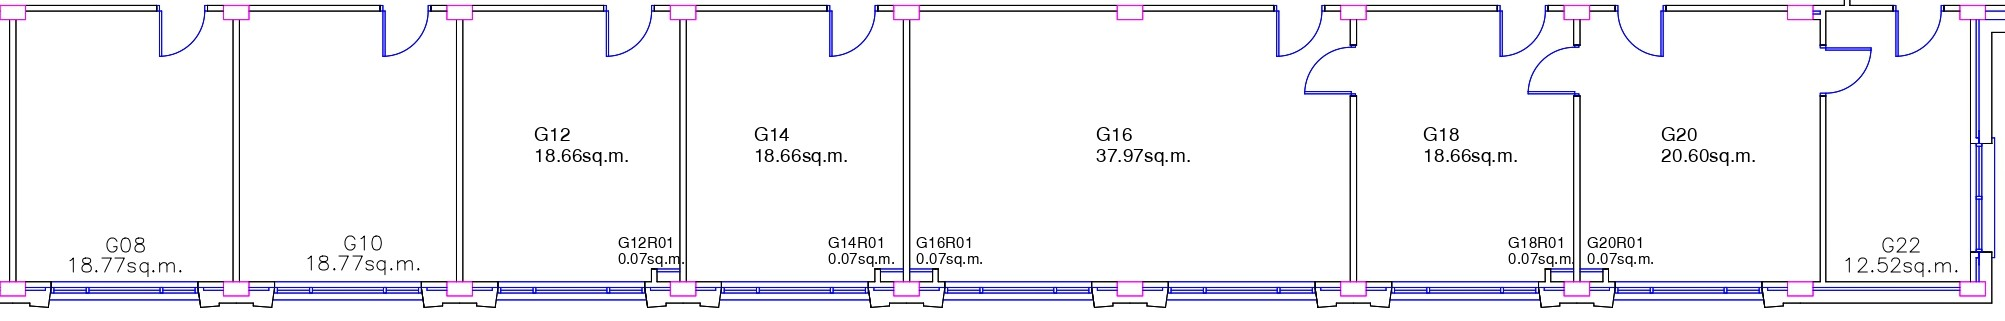
\includegraphics[width=\textwidth]{fig_case2_floor_plan_watson.jpg}
    \caption{Example floor layout of the Watson Building.}
    \label{fig_case2_watson}
\end{figure*}

We apply the selected data-driven methods to this real-world problem. Since no explicit objective functions are available, real evaluations cannot be conducted. To ensure comparability with existing works the experimental setup, including the optimization algorithm, room configuration, and indoor environmental settings, follows case study 2 in~\cite{building_opt2}, with the number of generations set to 200. The optimization results, including the obtained non-dominated solutions and the building layouts corresponding to the extremal solutions for each objective, are shown in Figures~\ref{fig_top1}, ~\ref{fig_top2} and ~\ref{fig_top3}. The HV values of the obtained fronts derived from surrogate-based evaluations, together with the objective improvements of the selected solutions, are shown in Table~\ref{tab:case_study_results}. Due to differences in the prediction ranges of the surrogate models, the HV values reported in the table are not directly comparable across methods, and the obtained fronts exhibit different patterns. These results should be interpreted within each method rather than compared directly across methods.

\begin{table*}[htbp]
\centering
\caption{HV values of the obtained fronts and comparison between the initial solution and selected obtained solutions in case study.}
\label{tab:case_study_results}
\scriptsize
\resizebox{\textwidth}{!}{
\begin{tabular}{llcccc}
\toprule
Surrogate + Optimizer & HV 
& Initial solution 
& Obtained solution A 
& Obtained solution B 
& Obtained solution C \\
\midrule

\multirow{2}{*}{TabPFN + NSGA-II} 
& \multirow{2}{*}{0.067}
& $f_{\mathrm{cost}} = 0.322$
& $f_{\mathrm{cost}} = 0.255$ $(+20.834\%)$
& $f_{\mathrm{cost}} = 0.262$ $(+18.465\%)$
& $f_{\mathrm{cost}} = 0.302$ $(+6.044\%)$ \\

& 
& $f_{\mathrm{tc}} = 0.586$
& $f_{\mathrm{tc}} = 0.663$ $(-13.033\%)$
& $f_{\mathrm{tc}} = 0.634$ $(-8.161\%)$
& $f_{\mathrm{tc}} = 0.521$ $(+11.206\%)$ \\

\midrule

\multirow{2}{*}{GPR-Mat\'ern + NSGA-II} 
& \multirow{2}{*}{0.086}
& $f_{\mathrm{cost}} = 0.209$
& $f_{\mathrm{cost}} = 0.191$ $(+8.321\%)$
& $f_{\mathrm{cost}} = 0.197$ $(+5.529\%)$
& $f_{\mathrm{cost}} = 0.207$ $(+0.661\%)$ \\

& 
& $f_{\mathrm{tc}} = 0.586$
& $f_{\mathrm{tc}} = 0.596$ $(-1.583\%)$
& $f_{\mathrm{tc}} = 0.546$ $(+6.943\%)$
& $f_{\mathrm{tc}} = 0.519$ $(+11.571\%)$ \\

\midrule

\multirow{2}{*}{GPR-Mat\'ern + Dual-Ranking NSGA-II} 
& \multirow{2}{*}{0.085}
& $f_{\mathrm{cost}} = 0.209$
& $f_{\mathrm{cost}} = 0.191$ $(+8.429\%)$
& $f_{\mathrm{cost}} = 0.195$ $(+6.369\%)$
& $f_{\mathrm{cost}} = 0.206$ $(+1.417\%)$ \\

& 
& $f_{\mathrm{tc}} = 0.586$
& $f_{\mathrm{tc}} = 0.606$ $(-3.289\%)$
& $f_{\mathrm{tc}} = 0.564$ $(+3.776\%)$
& $f_{\mathrm{tc}} = 0.522$ $(+10.962\%)$ \\

\bottomrule
\end{tabular}
}
\end{table*}

\begin{figure}[htbp]
\centering
\begin{overpic}[width=\linewidth]{tabpfn_pf.png}
    \put(35,67){TabPFN+NSGA-II}
    \put(51,0.78){$f_\mathrm{cost}$}
    \put(-2,34){$f_\mathrm{tc}$}
\end{overpic}
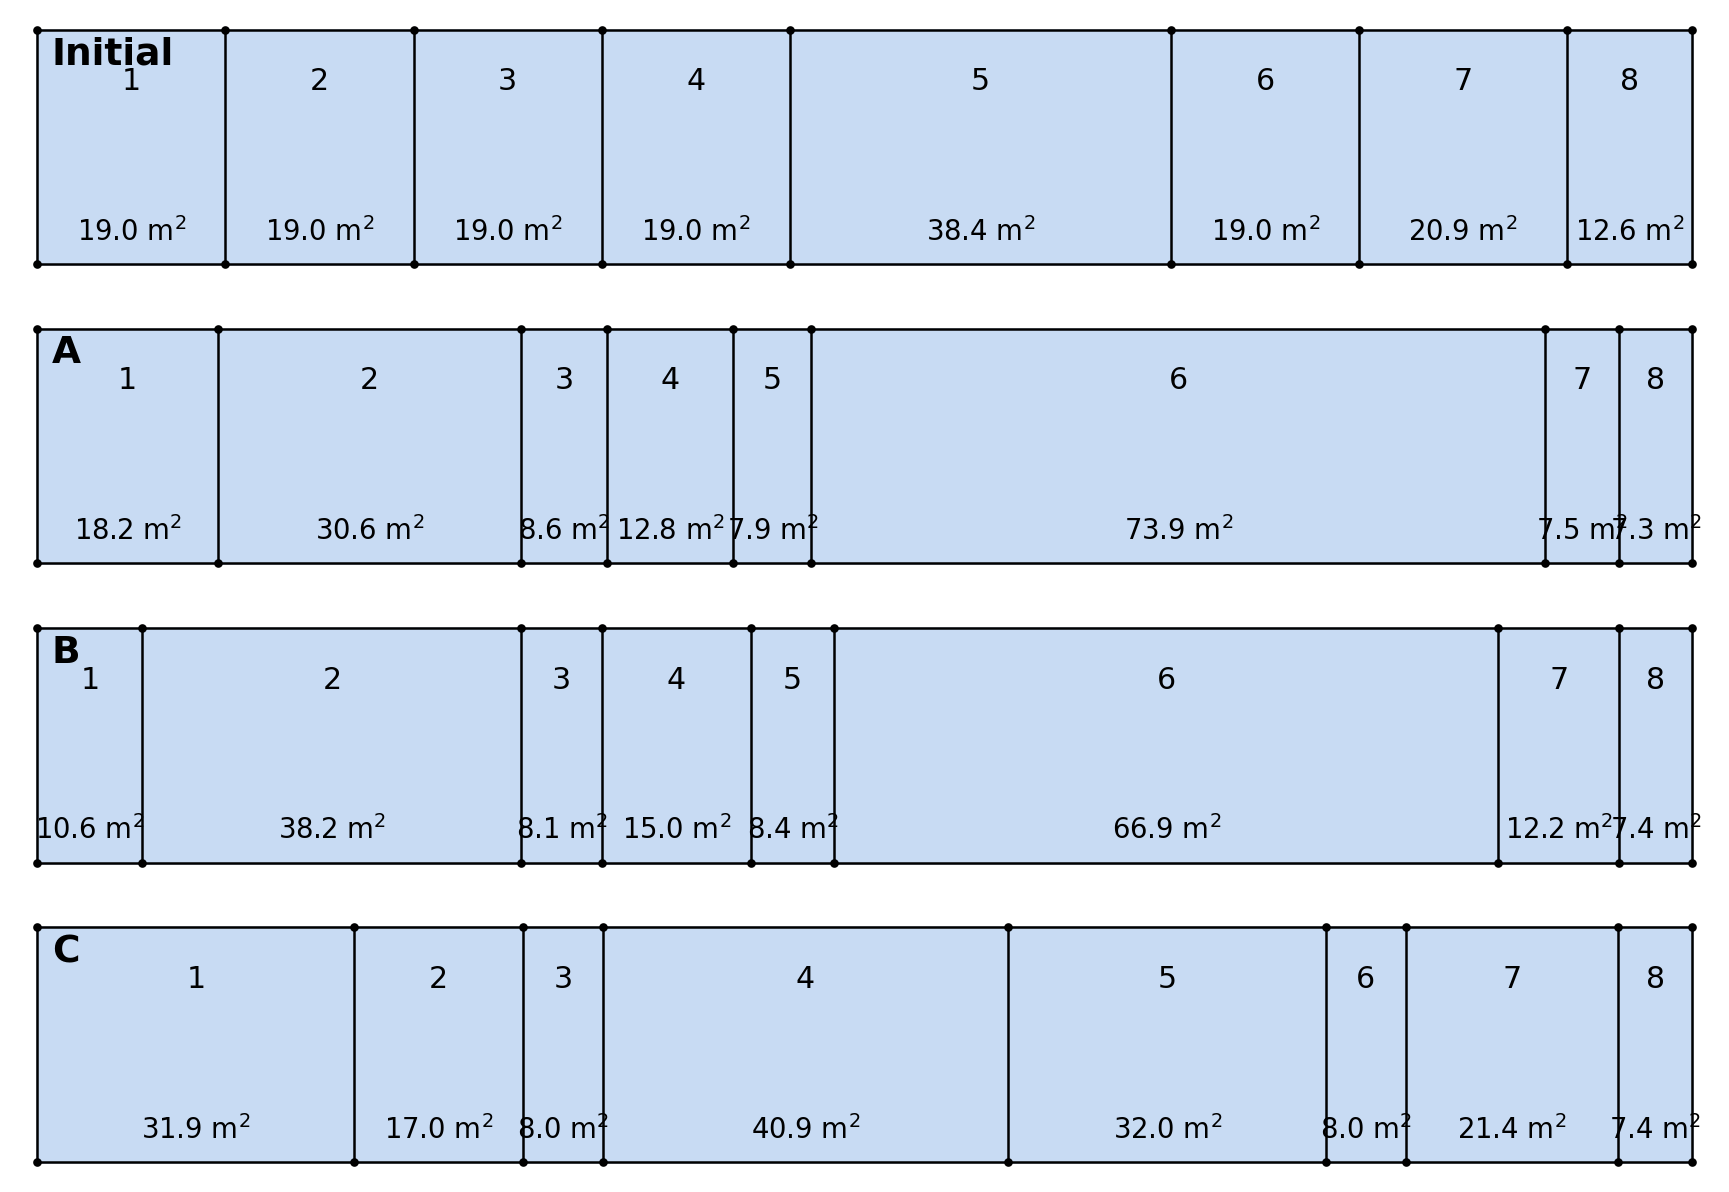
\includegraphics[width=\linewidth]{tabpfn_layout.png}
\caption{Top: Obtained front derived from the TabPFN+NSGA-II method. Bottom: Room layout solutions, with the initial layout and solutions A, B, and C arranged sequentially from top to bottom.}
\label{fig_top1}
\end{figure}

\begin{figure}[htbp]
\centering
\begin{overpic}[width=\linewidth]{gpr_matern_pf.png}
    \put(33,67){GPR-Mat\'ern+NSGA-II}
    \put(51,0.78){$f_\mathrm{cost}$}
    \put(-2,34){$f_\mathrm{tc}$}
\end{overpic}
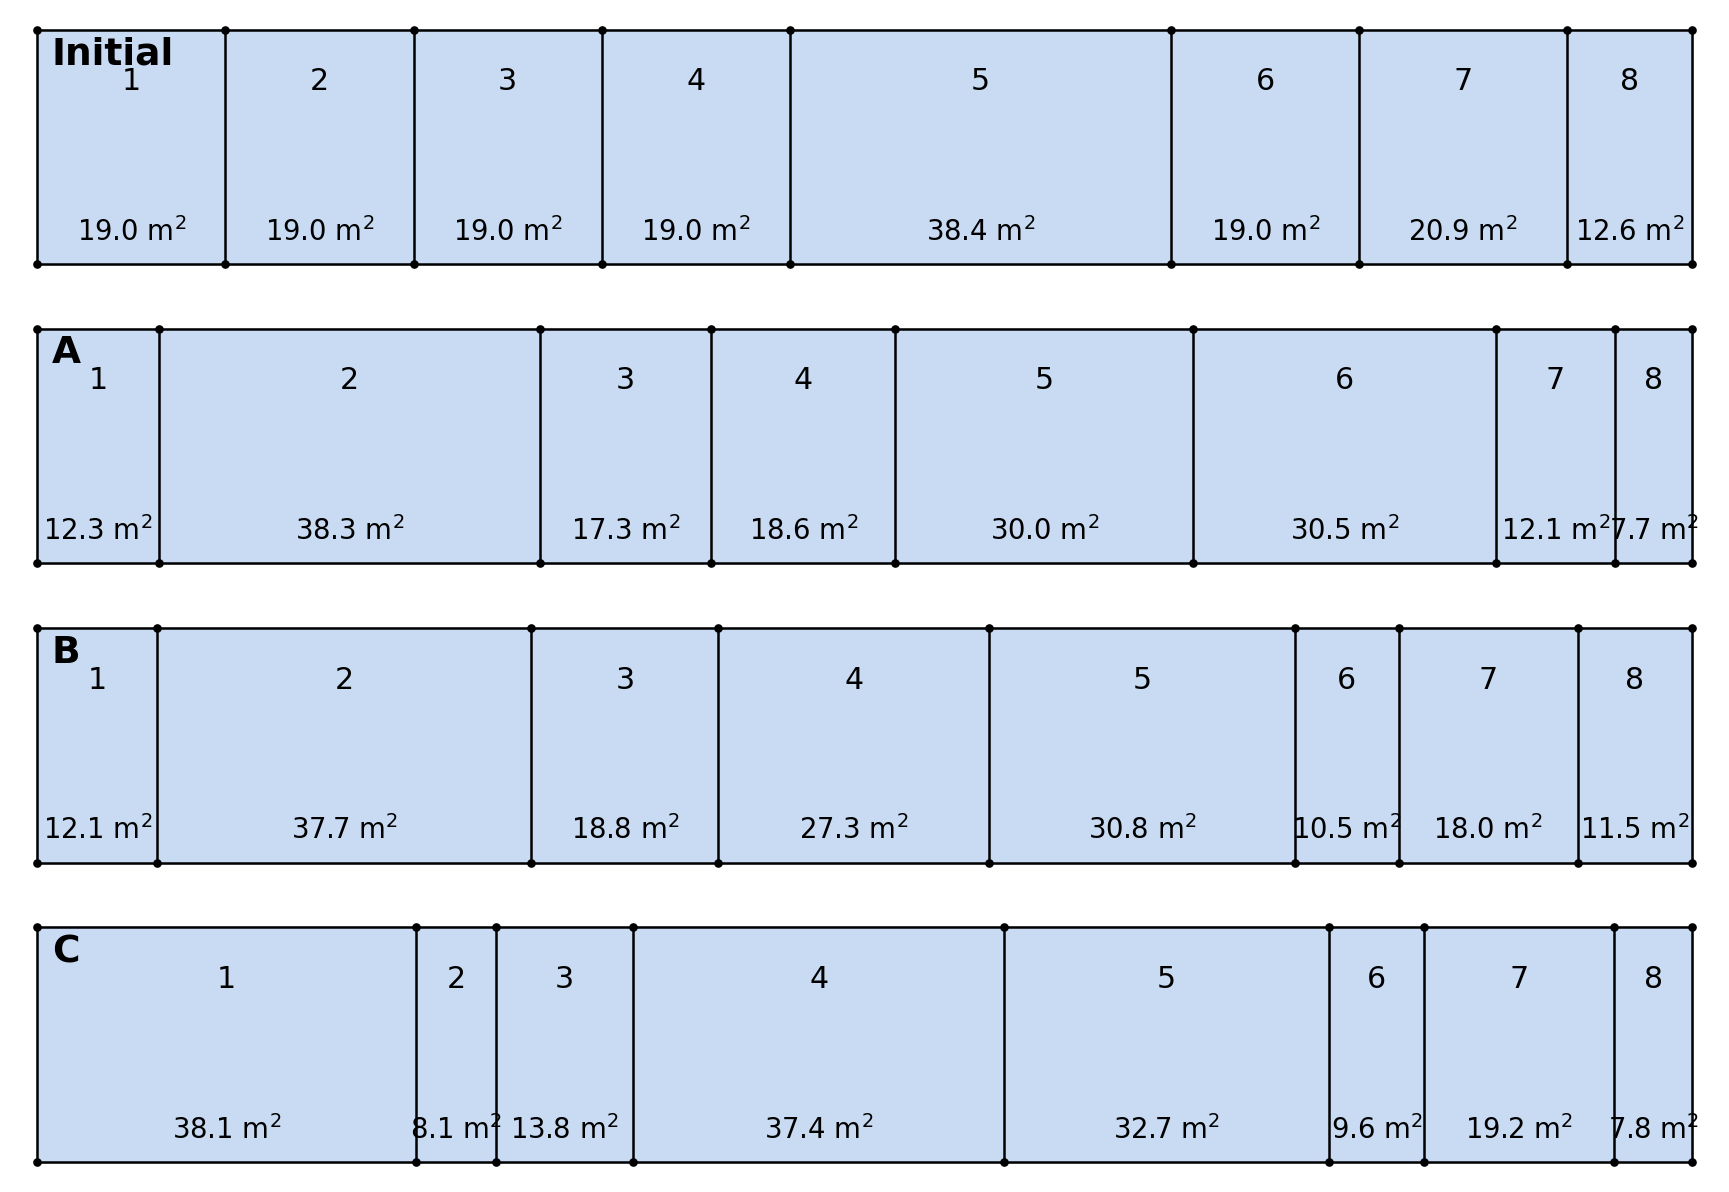
\includegraphics[width=\linewidth]{gpr_matern_layout.png}
\caption{Top: Obtained front derived from the GPR-Mat\'ern+NSGA-II method. Bottom: Room layout solutions, with the initial layout and solutions A, B, and C arranged sequentially from top to bottom.}
\label{fig_top2}
\end{figure}


\begin{figure}[htbp]
\centering
\begin{overpic}[width=\linewidth]{gpr_matern_dr_pf.png}
    \put(28,67){GPR-Mat\'ern+NSGA-II+DR}
    \put(51,0.78){$f_\mathrm{cost}$}
    \put(-2,34){$f_\mathrm{tc}$}
\end{overpic}
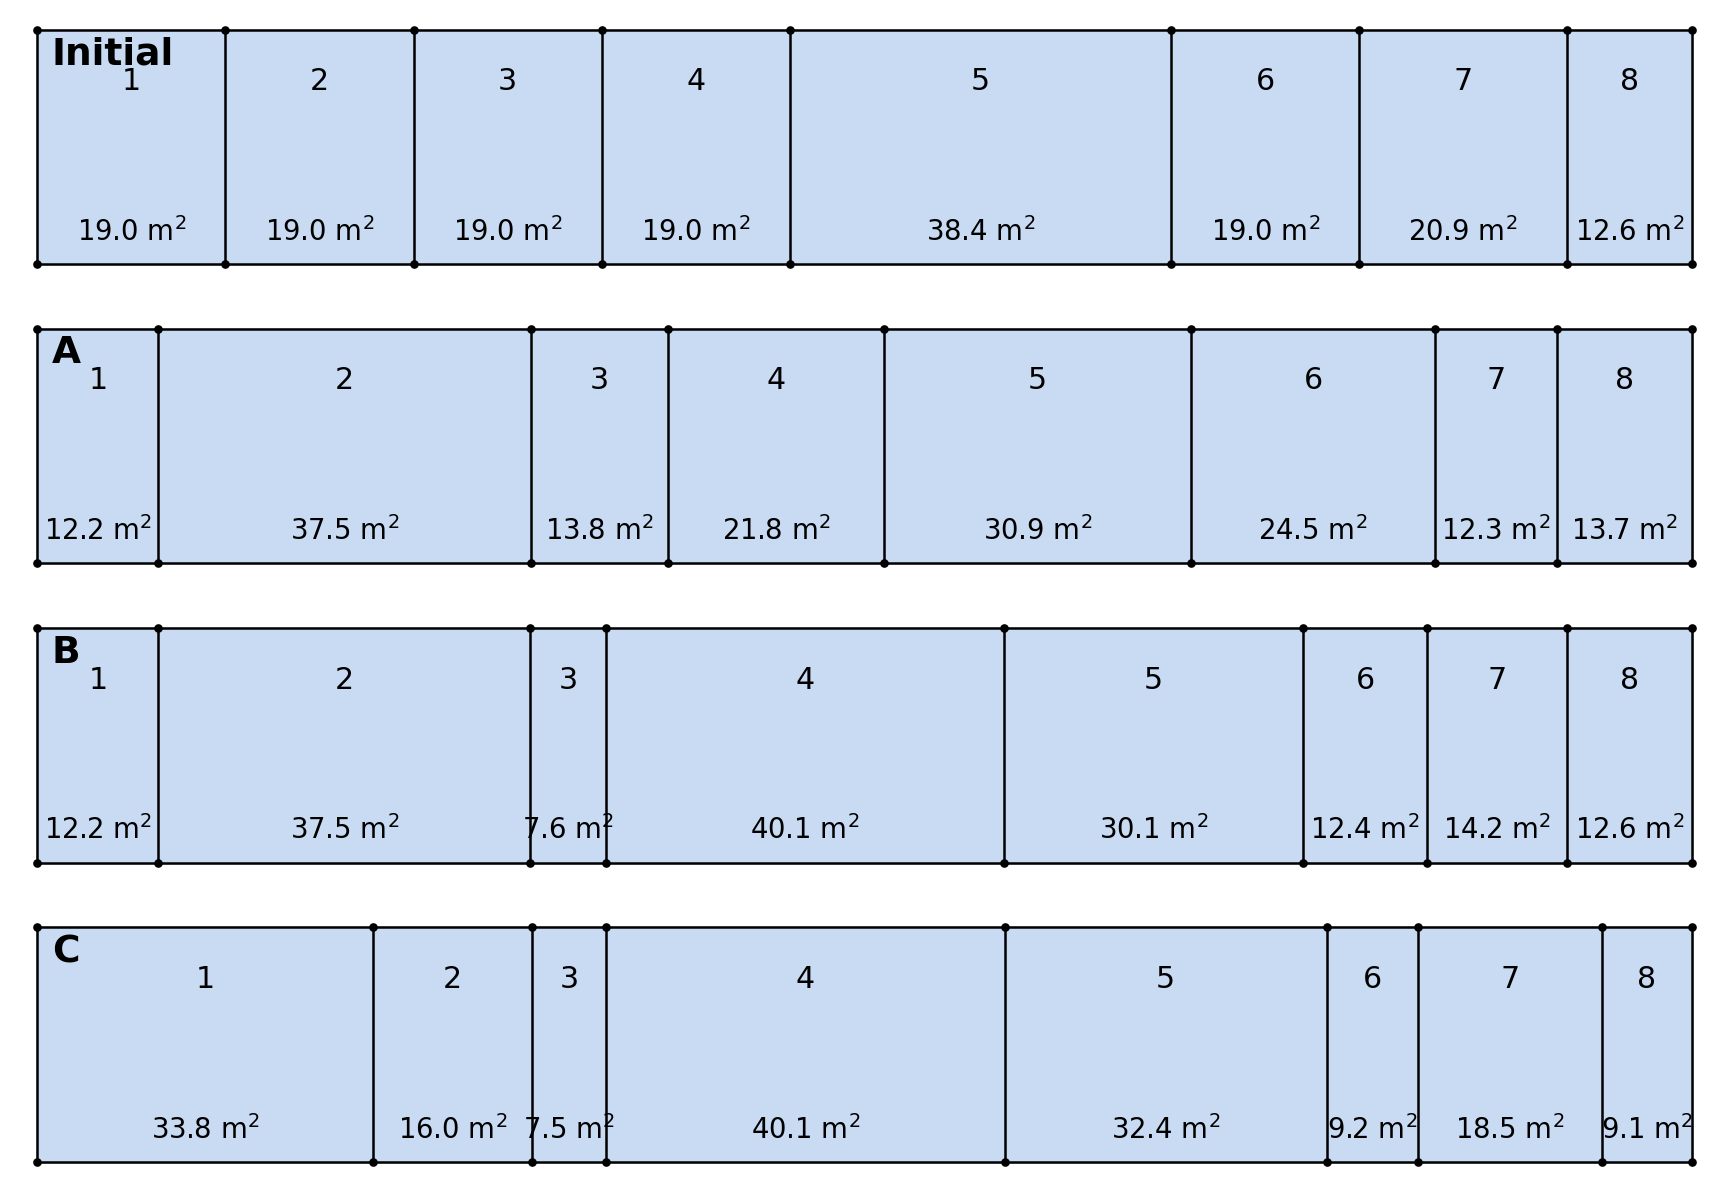
\includegraphics[width=\linewidth]{gpr_matern_dr_layout.png}
\caption{Top: Obtained front derived from the GPR-Mat\'ern+NSGA-II+DR method. Bottom: Room layout solutions, with the initial layout and solutions A, B, and C arranged sequentially from top to bottom.}
\label{fig_top3}
\end{figure}
For each method, solution A achieves the greatest energy savings, solution B represents a balanced solution, and solution C achieves the best thermal comfort. For TabPFN+NSGA-II, solution A achieves the largest cost reduction, improving $f_{\mathrm{cost}}$ by 20.834\%, but this is accompanied by a 13.033\% degradation in $f_{\mathrm{tc}}$. Solution B still provides a cost improvement of 18.465\%, although thermal comfort is also degraded by 8.161\%. Solution C improves $f_{\mathrm{tc}}$ by 11.206\% while maintaining a smaller cost improvement of 6.044\%. The corresponding layouts indicate that the cost-oriented TabPFN solutions tend to concentrate a large area in room 6 while reducing the areas of several other rooms, whereas the comfort-oriented solution allocates larger areas to rooms 1, 4, 5, and 7. For GPR-Mat\'ern+NSGA-II, the obtained front appears smoother. Solution A improves cost by 8.321\% with only a slight degradation in thermal comfort. Solution B improves both objectives, and solution C provides the largest thermal-comfort improvement of 11.571\% while preserving a small cost gain. The GPR-Mat\'ern+NSGA-II+DR method shows a relatively similar pattern. The layout results of the two GPR-based methods are also relatively consistent, with the cost-oriented and balanced solutions assigning larger areas to rooms 2, while the comfort-oriented solutions allocate more space to rooms 1, 4, and 5.


\section{Conclusion}
This paper conducts comparative experiments on eight real-world benchmark problems to evaluate offline data-driven \gls{MOEAs} for real-world applications. When only optimization performance is considered, TabPFN+NSGA-II performs best, followed by QR+NSGA-II+DR and WeightedEnsemble\L2+NSGA-II. When all metrics are considered jointly, TabPFN+NSGA-II remains the best-performing method, while the second and third methods change to GPR-Mat\'ern+NSGA-II and GPR-Mat\'ern+NSGA-II+DR, respectively. For the real-world building space optimization problem, the obtained solutions are not directly comparable across methods because the surrogate models produce different prediction ranges, which also leads to different patterns of obtained fronts. The optimized layout-results reveal some similar room-configuration patterns. Energy-saving solutions generally allocate more space to room 2, while comfort-oriented solutions tend to allocate more space to rooms 1, 4, 5, and 7.




\bibliographystyle{IEEEtran}
\bibliography{mybibfile}



\appendix
\section{Experiments}
\subsection{Experimental Settings}
The objective bounds used for min-max normalization before \gls{HV} calculation are reported in Table~\ref{tab_hv_objective_bounds}. 


\begin{table}[ht]
\caption{Objective bounds used for hypervolume normalization}
\centering
\begin{tabular}{lcc}
\toprule
Problem & Objective minimum & Objective maximum \\
\midrule
RE21 &(0, 0) &(2.971e+03, 4.855e-02) \\
RE22 &(0, -1.500e+03) &(8.291e+02, 1.200e+10) \\
RE23 &(0, 0) &(7.137e+05, 1.289e+06) \\
RE24 &(-1.000e+00, -1.000e+00) &(6.000e+03, 1.000e+02) \\
RE25 &(-1.000e+01, -6.000e+04) &(1.248e+02, 1.004e+07) \\
MO-Portfolio &(0, -5.000e-01) &(2.941e-01, -1.362e-01) \\
Truss2D &(0, 0) &(6.000e-02, 1.500e+10) \\
Welded Beam &(0, -2.000e+02) &(3.000e+02, 1.600e+02) \\
\bottomrule
\end{tabular}
\label{tab_hv_objective_bounds}
\end{table}



\end{document}
